\documentclass{article}   % Spesifikasi Kelas Dokumen
% ==================== Pengaturan Dokumen ====================
\usepackage{amsmath}  % For math
\usepackage{amssymb}  % For more math
\usepackage{enumerate} % useful for itemization
\usepackage{enumitem}
\usepackage{siunitx}  % standardization of si units
\usepackage{graphicx}
\usepackage{lipsum}
\graphicspath{{./gambar/}} %picture path
\usepackage{pgfplots}
\pgfplotsset{compat = newest}

%Stop indentation on new paragraphs
\usepackage[parfill]{parskip}
\usepackage[numbers]{natbib}
% Since natbib uses an unnumbered section by default we define \bibsection
% to make it a regular numbered section.
\renewcommand\bibsection{\section{Daftar Pustaka}}
\bibliographystyle{ieeetr}
%citecolor
\usepackage[colorlinks,linkcolor={black},citecolor={blue!80!black},urlcolor={blue!80!black}]{hyperref}

\usepackage{lastpage}
\usepackage{setspace}
\usepackage{xcolor}
\usepackage{geometry}
\geometry{
	a4paper,
	%total={170mm,257mm},
	left=25mm,
	right=20mm,
	top=25mm,
	bottom=20mm,
}

%=================== Untuk Header dan Footer===================

\newcommand{\nama}{Zaitun,S.Si.,M.Mat}
\newcommand{\judul}{Judul Artikel}
\newcommand{\judulfooter}{\emph{Judul}}
\newcommand{\versi}{2023 v1.01}
\newcommand{\asosiasi}{Institut Teknologi Bacharuddin Jusuf Habibie}

\usepackage{fancyhdr}
\pagestyle{fancy}
%  --------   Normal Headers
\fancyhf{} % clear all fields
\fancyhead[L]{\asosiasi}
\fancyfoot[L]{\nama,~\judulfooter}
\fancyfoot[R]{\textsf{Tulisan \versi~pages \textsf{\thepage~of~\pageref{LastPage}}}}
\renewcommand{\headrulewidth}{1pt} % to remove line on header
\renewcommand{\footrulewidth}{1pt} % to remove line on footer

%=====================MULAI DOKUMEN=====================

\begin{document}
\begin{center}
    \vspace{.4cm}
    {\textbf { \huge \judul}}\\ [0.5cm]
    \textsf{\large \nama}\\[0.1cm]
    \text{\asosiasi}
\end{center}
\vspace{.4cm}
\hrule
\vspace{.4cm}

\begin{center}
	\textbf{\Large - Pengantar -}
\end{center}
\paragraph*{} 
\lipsum[2]
\section{Judul 1 }
\thispagestyle{empty} %Clear Header and Footer

\paragraph*{} 
\lipsum[2-3]

\subsection{Judul 1 1}
\lipsum[4]
\begin{figure*} [h]
	\centering
	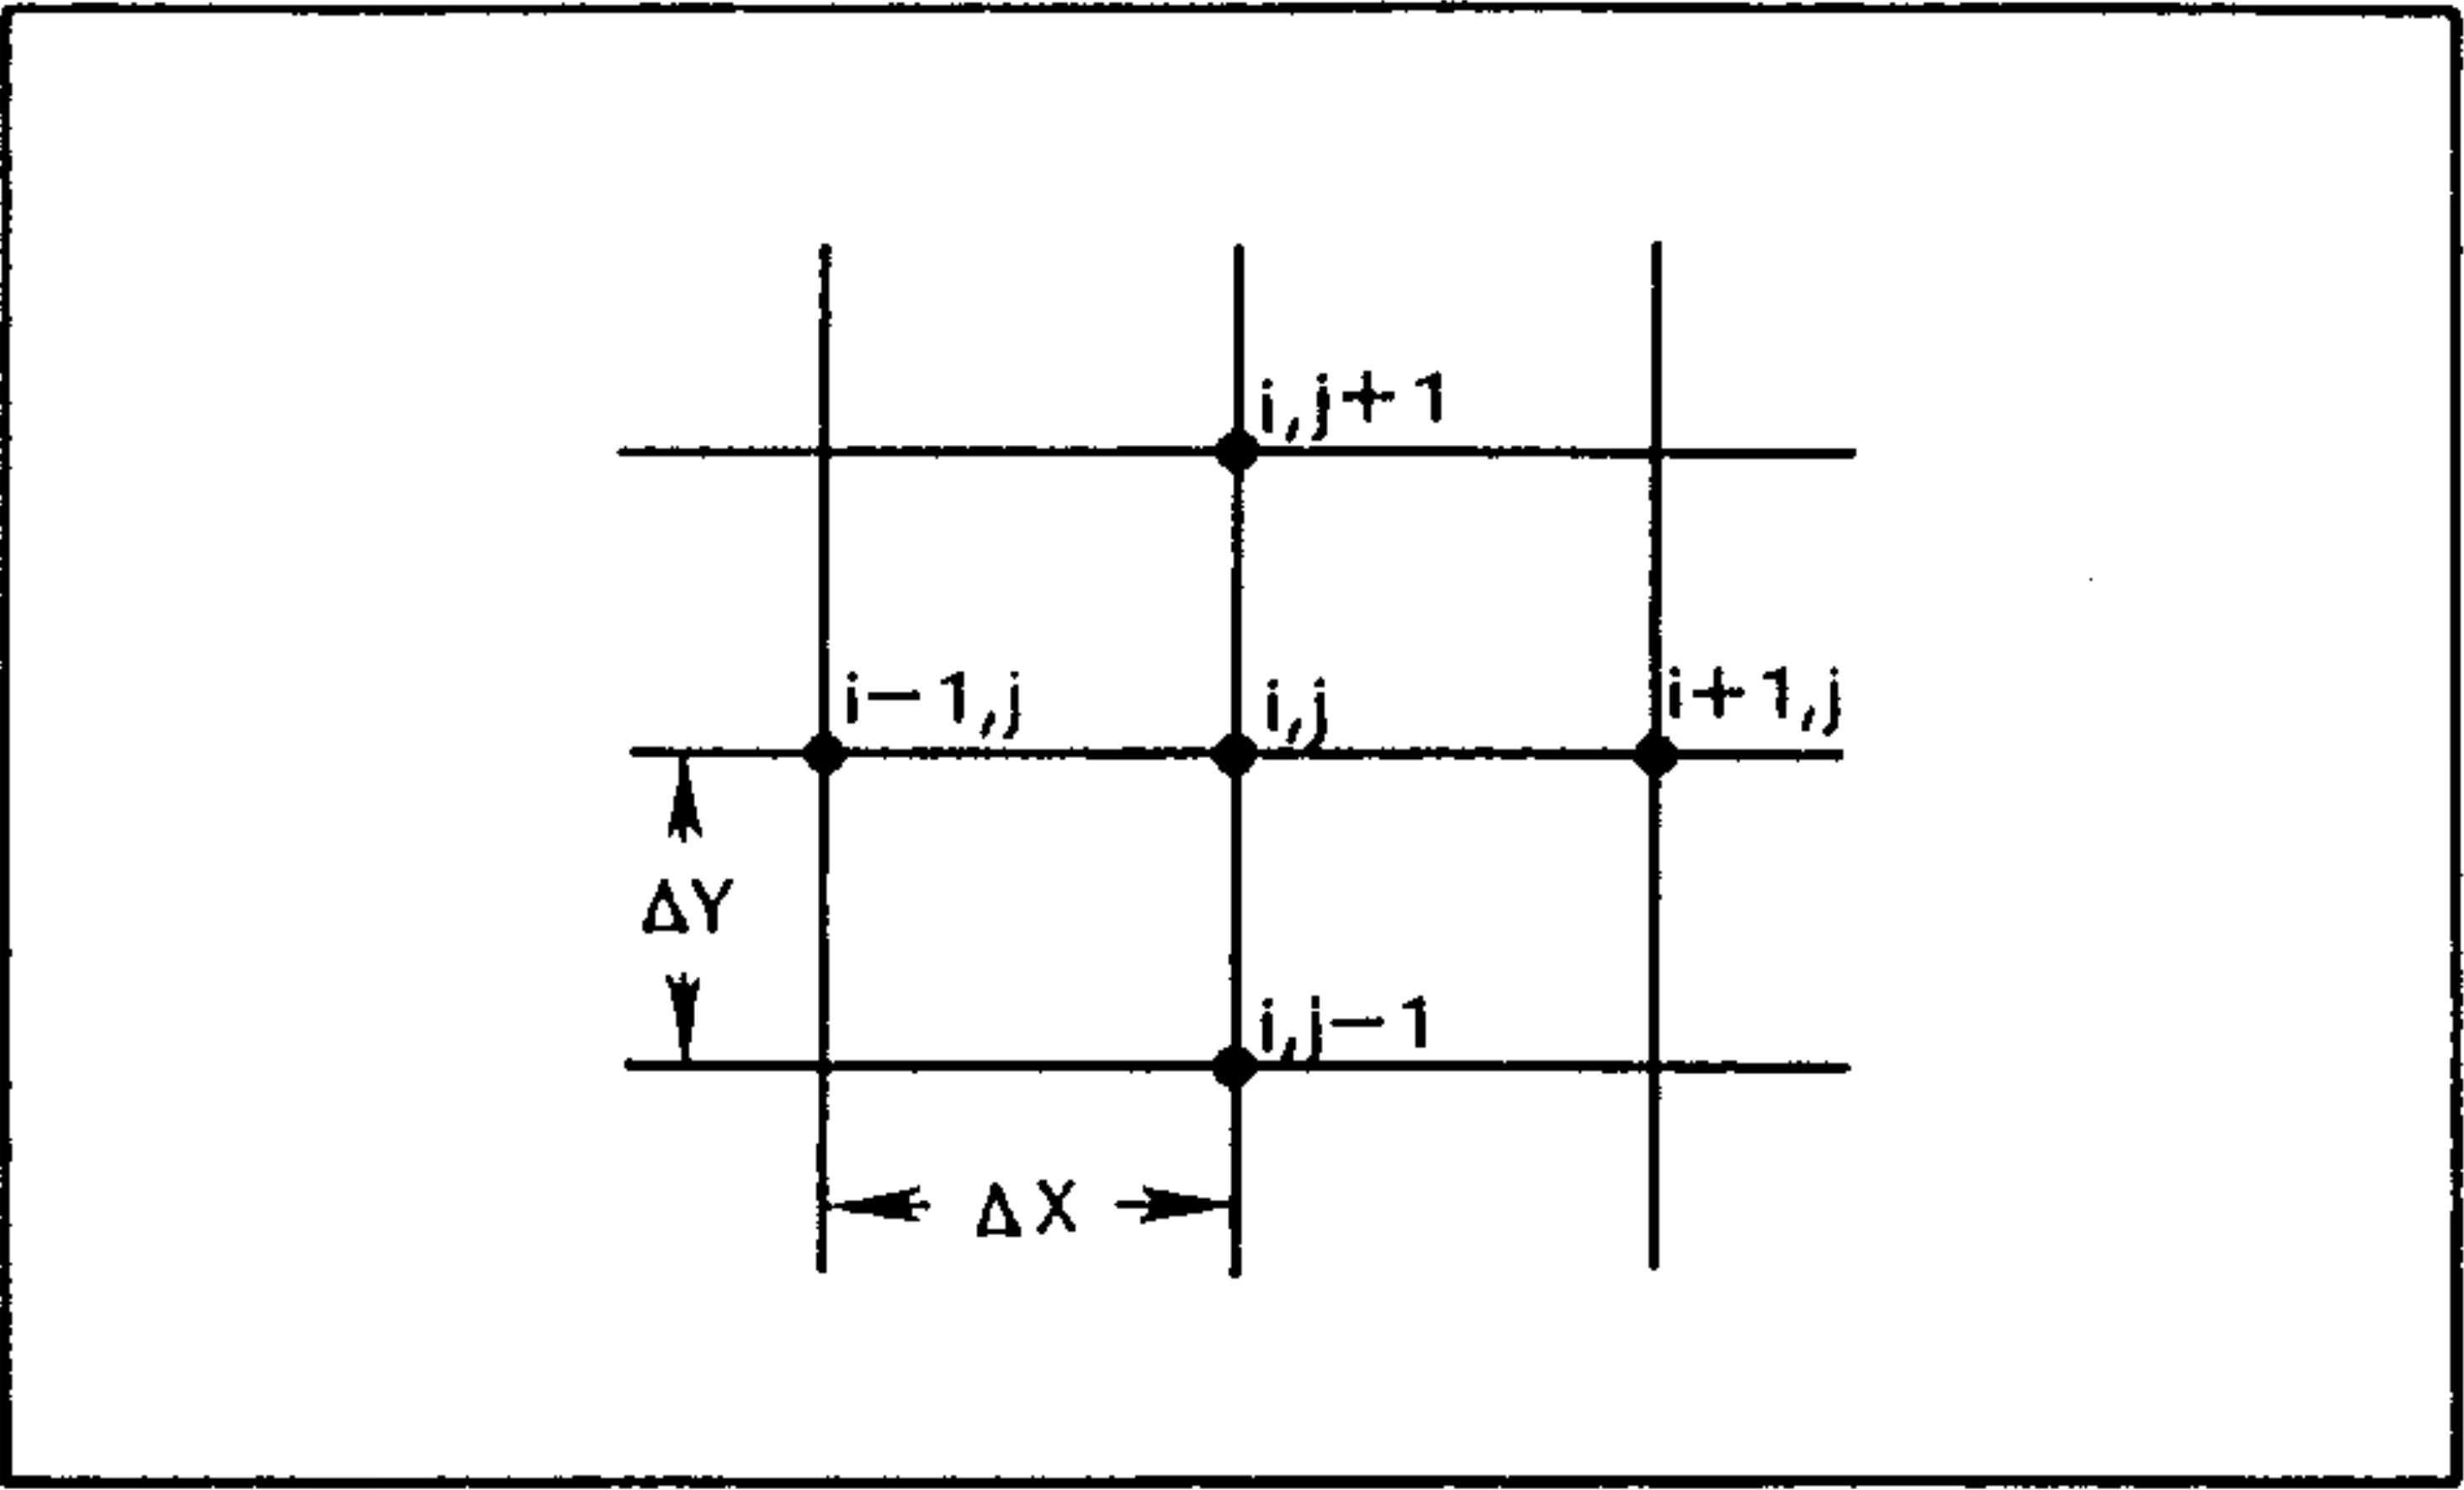
\includegraphics[height=0.2\paperwidth]{1.png}
	\caption{Titik grid formulasi numerik \textbf{\cite{hoff153}}}
	\label{G01}
\end{figure*}\\

\subsubsection{Judul 111}
\lipsum[4-5]
\begin{figure*}[h]
	\centering
	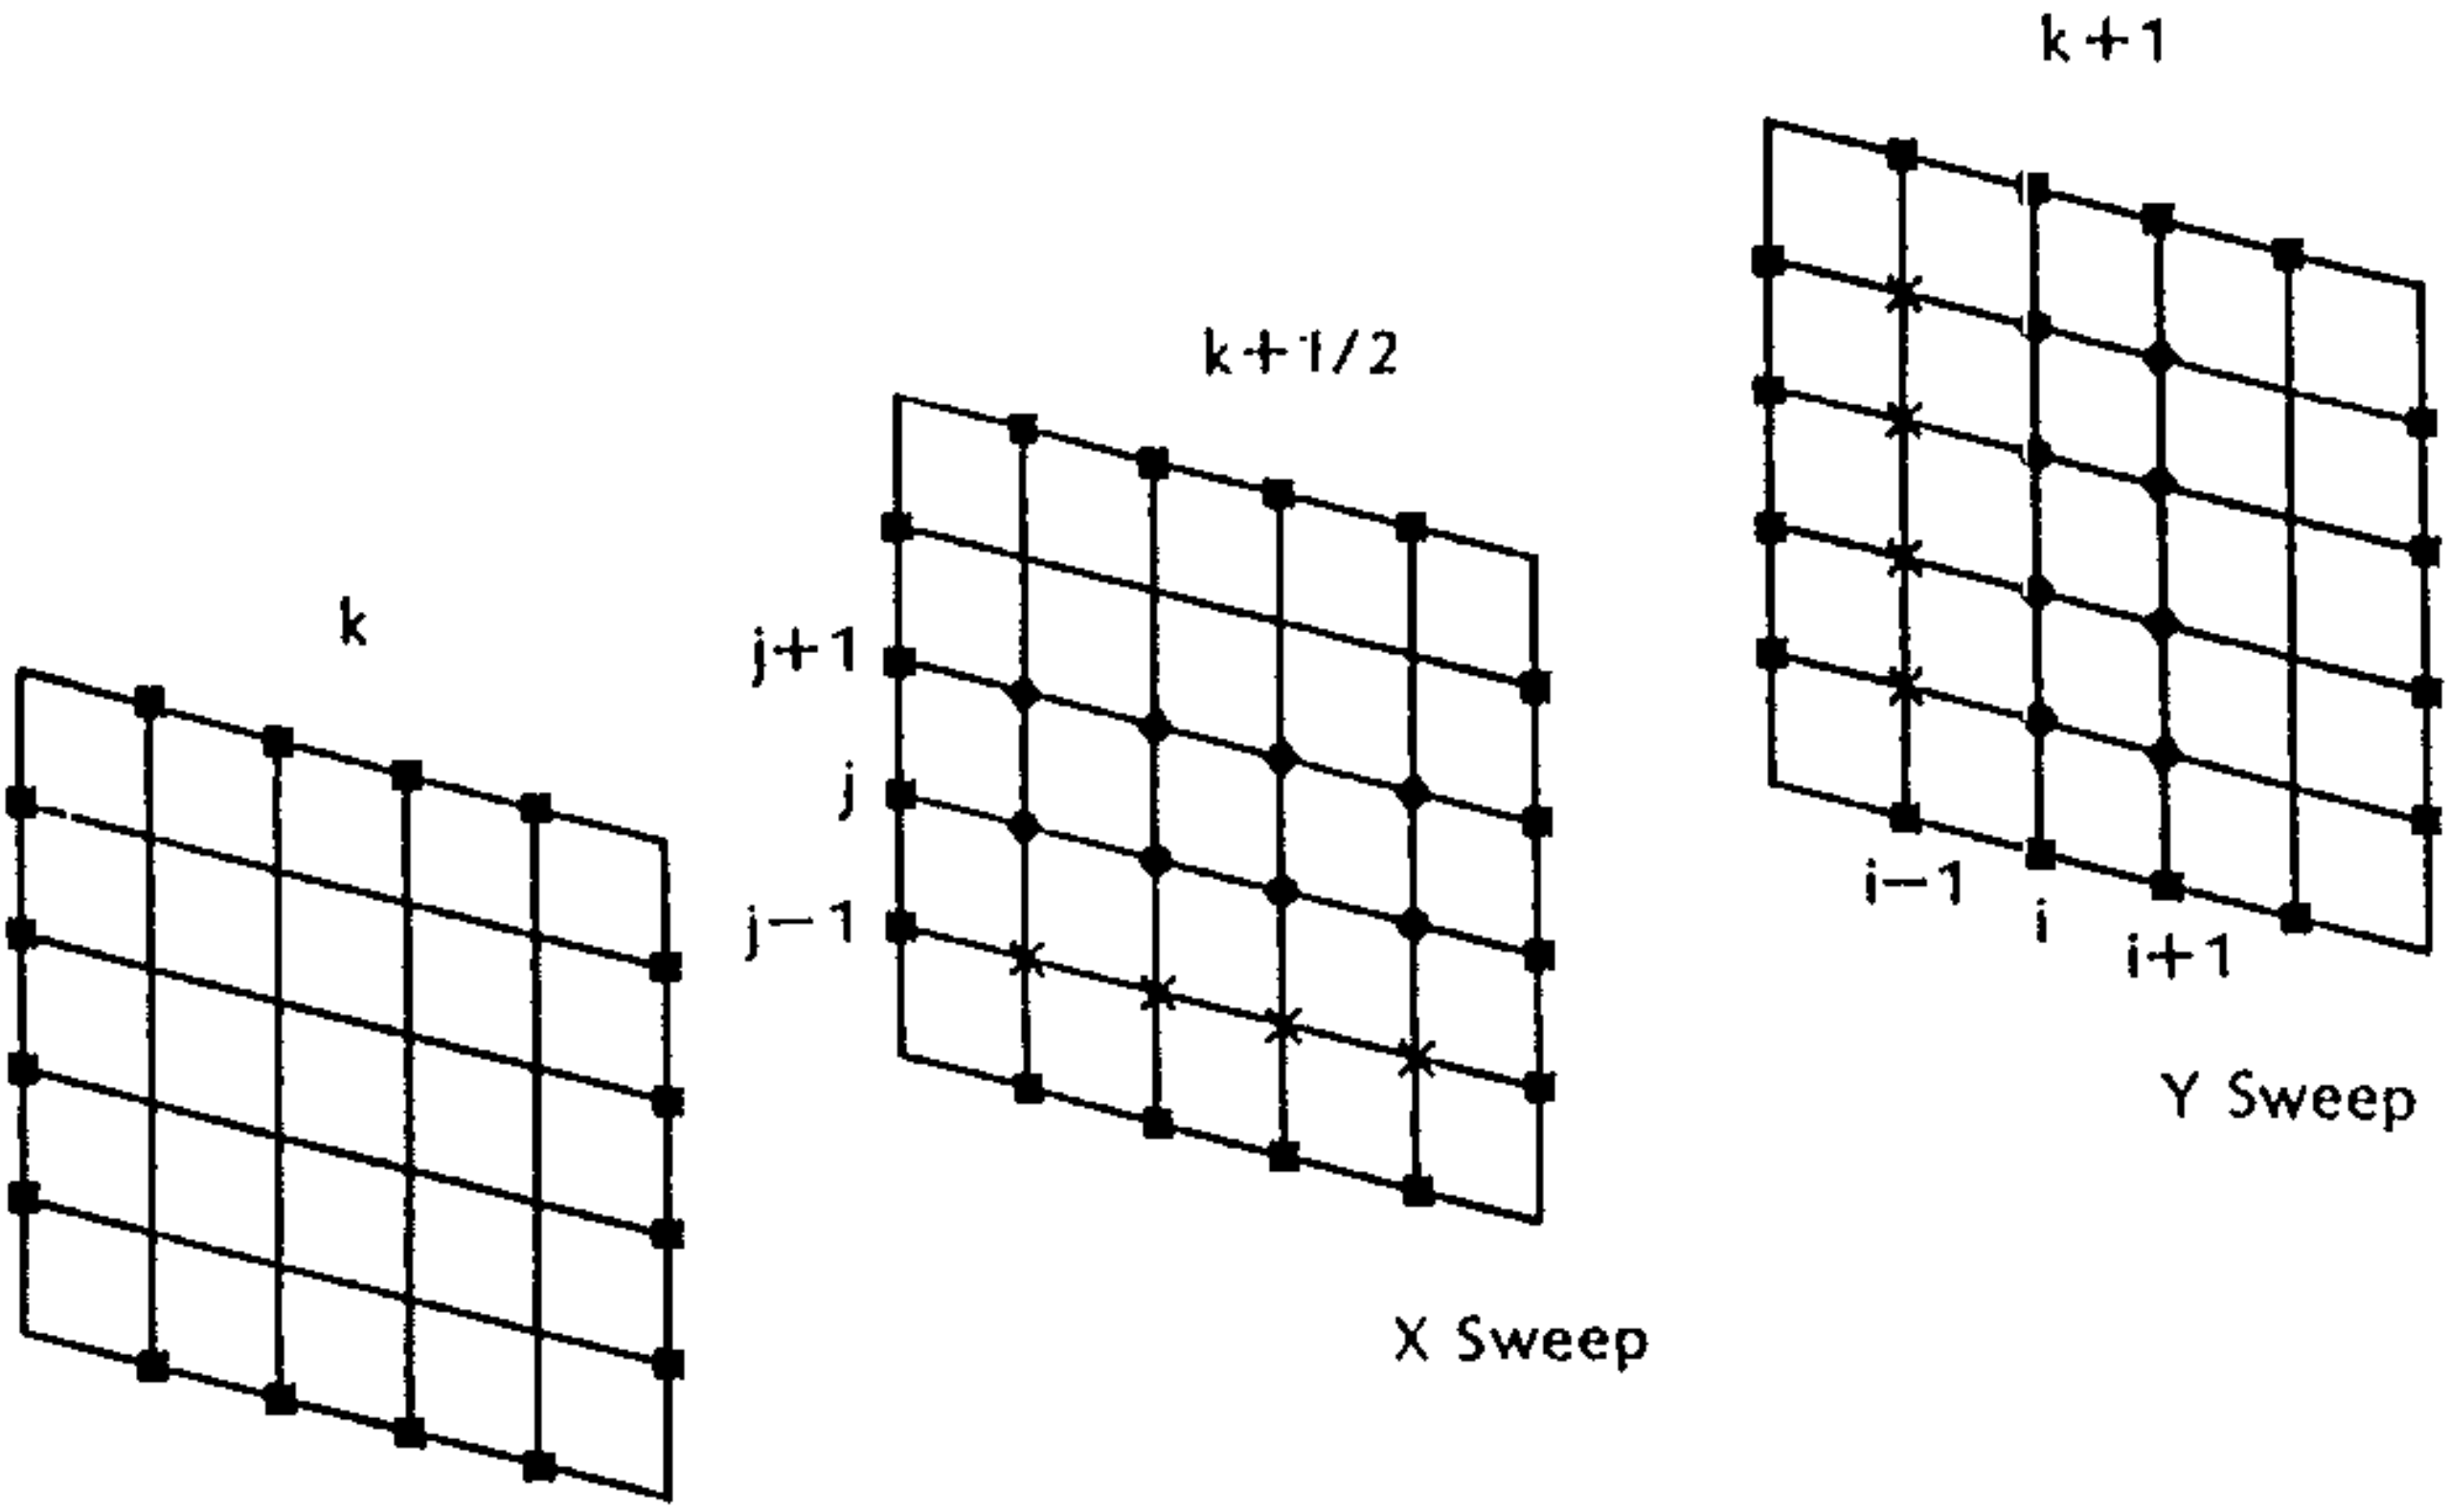
\includegraphics[height=0.25\paperwidth]{2.png}
	\caption{Proses langkah pengerjaan metode ADI \textbf{\cite{hoff166}}}
	\label{G02}
\end{figure*}

\subsection{Judul 1 2}
\lipsum[5-7]
\subsubsection{Judul 1 2 1}
\lipsum[8]
\section{Kesimpulan}
\paragraph*{} \lipsum[9].\cite{fahim,gos,hoff,hoff153,hoff166,Keshav,subiono}
	\section{Tugas Mandiri}
\begin{enumerate}
	\item Tentukan luas daerah apabila daerah tersebut dibatasi oleh fungsi $ {\displaystyle f(x)=-(x-0.5)^2+2 }$, $ {\displaystyle g(x)=\frac{2}{3}x}$, serta garis $ x=0 $ dan $ x=1 $. Kemudian gambarkan grafik dari daerah tersebut.%1
	\item Hitunglah nilai integral berikut%2
	\begin{align*}
		\int_{0}^{1}-2x^{4/3} + 2x^{1/3} \,dx &= \left[-\dfrac{6}{7}x^{\frac{7}{3}}+\frac{3}{2}x^{\frac{4}{3}} \right]_{0}^{1}
	\end{align*} 
	\item Hitunglah nilai integral berikut\\ %3
	\begin{align*}
		\int_{-2}^{-1}(2x+2)(x^2+2x) \,dx  &= \int_{x=-2}^{x=-1}(x^2+2x) \,d(x^2+2x)
	\end{align*} 
\end{enumerate}

\bibliography{section/references}

	\begin{center}
		\section*{Lampiran}
	\end{center}
	\textbf{{Persamaan Laplace 2D}}\\
Diberikan persamaan Laplace berikut
$$ \dfrac{\partial^2 u}{\partial x^2} + \dfrac{\partial^2 u}{\partial y^2}= 0, ~~ 0\leq x \leq 1,~~ 0\leq y \leq 1$$
$$ u(0,y)=10, ~~u(1,y)=0, ~~ u(x,0)=0, ~~u(x,1)=0$$
Dengan menerapkan metode beda hingga ADI didapatkan persamaan berikut
$$ \dfrac{\partial^2 u}{\partial x^2} + \dfrac{\partial^2 u}{\partial y^2}= \dfrac{\partial}{\partial x}\left ( \dfrac{\partial u}{\partial x}\right )+\dfrac{\partial}{\partial y}\left ( \dfrac{\partial u}{\partial y}\right )$$
dengan pendekatan metode beda hingga dengan langkah waktu $ \frac{1}{2} $ persamaan di atas akan didekati dengan
\begin{align*}
	\dfrac{\partial}{\partial x} \left. \dfrac{\partial u}{\partial x} \right |_{i,j}^{n+\frac{1}{2}}+ \dfrac{\partial}{\partial y} \left. \dfrac{\partial u}{\partial y} \right |_{i,j}^{n+\frac{1}{2}} & \approx 
	\dfrac{\partial}{\partial x} \left( \dfrac{u_{i+1,j}^{n} - u_{i,j}^{n}}{\Delta x}+O(\Delta x,\Delta y)\right) + 
	\dfrac{\partial}{\partial y} \left( \dfrac{u_{i,j+1}^{n} - u_{i,j}^{n}}{\Delta y}+O(\Delta x,\Delta y) \right) \\
	&\approx 
	\dfrac{1}{\Delta x} \left( \left( \dfrac{u_{i+1,j}^{n}-u_{i,j}^{n}} {{\Delta x}}\right)  - \left( \dfrac{u_{i,j}^{n}-u_{i-1,j}^{n}} {{\Delta x}}\right)+O(\Delta x,\Delta y) \right) -O(\Delta x,\Delta y)+ \\
	&~~~~\dfrac{1}{\Delta y} \left( \left( \dfrac{u_{i,j+1}^{n}-u_{i,j}^{n}}{{\Delta y}}\right)  - \left( \dfrac{u_{i,j}^{n}-u_{i,j-1}^{n}}{{\Delta y}}-O(\Delta x,\Delta y)\right) +O(\Delta x,\Delta y)\right) \\
	& \approx 
	\left( \dfrac{u_{i+1,j}^{n} - 2u_{i,j}^{n}+u_{i-1,j}^{n}}{(\Delta x)^2}\right) + 
	\left( \dfrac{u_{i,j+1}^{n} - 2u_{i,j}^{n}+u_{i,j-1}^{n}}{(\Delta y)^2}\right) =0
\end{align*}
\textbf{{Persamaan Difusi 2D}}\\
Diberikan persamaan difusi berikut
\begin{align}
	\dfrac{\partial u}{\partial t}= D_x\dfrac{\partial^2 u}{\partial x^2} + D_y \dfrac{\partial^2 u}{\partial y^2}, ~~ 0\leq x \leq 1,~~ 0\leq y \leq 1 \label{d1}
\end{align}
$$ \dfrac{\partial u}{\partial n}=0 \mid n=\{x,y\},~~u(0.5,0.5,t)=10\mid 0\leq t \leq 5, ~~u(x,y,0)=0 \mid (x,y)\neq (0.5,0.5),~~t\geq 0$$
Dengan menerapkan metode beda hingga dengan beda mundur pada grid waktu dan beda tengah pada grid ruang, sehingga didapatkan persamaan-persamaan berikut
\begin{align}
	\left. \dfrac{\partial u}{\partial t} \right |_{i,j}^{n} \approx \dfrac{u_{i,j}^{n}-u_{i,j}^{n-1}}{\Delta t}+O(\Delta t) \label{d2} \\
	\left.  \dfrac{\partial^2 u}{\partial x^2} \right |_{i,j}^{n} \approx \dfrac{u_{i+1,j}^{n} - 2u_{i,j}^{n}+u_{i-1,j}^{n}}{(\Delta x)^2} + O(\Delta x)^2 \label{d3}\\
	\left. \dfrac{\partial^2 u}{\partial y^2} \right |_{i,j}^{n} \approx 
	\dfrac{u_{i,j+1}^{n} - 2u_{i,j}^{n} + u_{i,j-1}^{n}}{(\Delta y)^2} + O(\Delta y)^2 \label{d4}
\end{align}

kemudian Persamaan (\ref{d2}) - (\ref{d4}) di substitusi ke Persamaan (\ref{d1}) dan menghilangkan notasi kesalahan pemotongan maka didapatkan persamaan berikut 
\begin{align*}
	\dfrac{u_{i,j}^{n}-u_{i,j}^{n-1}}{\Delta t} = D_x \dfrac{u_{i+1,j}^{n} - 2u_{i,j}^{n} + u_{i-1,j}^{n}}{(\Delta x)^2} + D_y \dfrac{u_{i,j+1}^{n} - 2u_{i,j}^{n} + u_{i,j-1}^{n}}{(\Delta y)^2} \\
	u_{i,j}^{n} - u_{i,j}^{n-1}  = \left(\dfrac{\Delta t D_x}{(\Delta x)^2} \right) \left( u_{i+1,j}^{n} - 2u_{i,j}^{n} + u_{i-1,j}^{n}\right) + \left( \dfrac{\Delta t D_y}{(\Delta y)^2}\right) \left( u_{i,j+1}^{n} - 2u_{i,j}^{n} + u_{i,j-1}^{n}\right)
\end{align*}
dengan menyusun kembali persamaan di atas maka didapatkan
\begin{align}
	\left(1+2A+2B \right)  u_{i,j}^{n} - A \left( u_{i+1,j}^{n} + u_{i-1,j}^{n}\right) - B \left( u_{i,j+1}^{n}  + u_{i,j-1}^{n}\right) = u_{i,j}^{n-1} \label{d5}
\end{align}
dengan $ A=\dfrac{\Delta t D_x}{(\Delta x)^2} $ dan $ B=\dfrac{\Delta t D_y}{(\Delta y)^2} $

\textbf{{Contoh Soal}}
\begin{enumerate}
	\item Hitunglah nilai integral berikut\\ %1
	\textbf{Jawaban;}
	\begin{align*}
		\int_{-2}^{1}3x^2+2 \,dx &= \left[x^3+2x \right]_{-2}^{1} \\
		&= [(1)^3+2(1)]-[(-2)^3+2(-2)] \\
		&= [3]-[-8-4]\\
		&= 15
	\end{align*} 
	\item Hitunglah nilai integral berikut \\ %2
	\textbf{Jawaban;}
	\begin{align*}
		\int_{0}^{1}-2x^{4/3} + 2x^{1/3} \,dx &= \left[-\dfrac{6}{7}x^{\frac{7}{3}}+\frac{3}{2}x^{\frac{4}{3}} \right]_{0}^{1} \\
		&= \left[-\dfrac{6}{7}(1)^{\frac{7}{3}}+\frac{3}{2}(1)^{\frac{4}{3}} \right]
		-\left[-\dfrac{6}{7}(0)^{\frac{7}{3}}+\frac{3}{2}(0)^{\frac{4}{3}} \right] \\
		&= \dfrac{9}{14}
	\end{align*} 
	\item Hitunglah nilai integral berikut\\ %3
	\textbf{Jawaban;}
	\begin{align*}
		\int_{-2}^{-1}(2x+2)(x^2+2x) \,dx  &= \int_{x=-2}^{x=-1}(x^2+2x) \,d(x^2+2x) \\
		&= \left[ \frac{1}{2}(x^2+2x)^2 \right]_{-2}^{-1} \\
		&= \left[\frac{1}{2}((-1)^2+2(-1))^2\right]-\left[\frac{1}{2}((-2)^2+2(-2))^2\right] \\
		&= \dfrac{1}{2}
	\end{align*} 
	\item Hitunglah nilai integral berikut\\ %4
	\textbf{Jawaban;}
	\begin{align*}
		\int_{\pi/6}^{\pi}2 \sin x \,dx  &= \left[-2 \cos x \right]_{\pi/6}^{\pi} \\
		&= [-2 \cos (\pi)]-[-2 \cos (\pi/6)] \\
		&= [2]-[-2(1/2\sqrt{3})]\\
		&= 2+\sqrt{3}
	\end{align*} 
	\item Tentukan luas daerah apabila daerah tersebut dibatasi oleh fungsi $ {\displaystyle f(x)=-(x-0.5)^2+2 }$, $ {\displaystyle g(x)=\frac{2}{3}x}$, serta garis $ x=0 $ dan $ x=1 $. Kemudian gambarkan grafik dari daerah tersebut.\\ %5
	\textbf{Jawaban;}
	\begin{align*}
		\int_{0}^{1}\left[ -(x-0.5)^2+2 \right] - \left[ \frac{2}{3}x\right] \,dx &=\int_{0}^{1}\left[ -x^2 + \frac{1}{3}x+\dfrac{7}{4} \right] \,dx\\
		&= \left[-\dfrac{1}{3}x^3 + \dfrac{1}{6}x^2 +\dfrac{7}{4}x \right]_{0}^{1} \\
		&= \left[-\dfrac{1}{3}(1)^3 + \dfrac{1}{6}(1)^2 +\dfrac{7}{4}(1) \right]- \left[-\dfrac{1}{3}(0)^3 + \dfrac{1}{6}(0)^2 +\dfrac{7}{4}(0) \right] \\
		&= \dfrac{19}{12} \text{ satuan luas}
	\end{align*} 
	\item Hitunglah nilai integral berikut\\ %1
	\textbf{Jawaban;}
	\begin{align*}
		\int_{-2}^{1}3x^2+2 \,dx &= \left[x^3+2x \right]_{-2}^{1} \\
		&= [(1)^3+2(1)]-[(-2)^3+2(-2)] \\
		&= [3]-[-8-4]\\
		&= 15
	\end{align*} 
	\item Hitunglah nilai integral berikut \\ %2
	\textbf{Jawaban;}
	\begin{align*}
		\int_{0}^{1}-2x^{4/3} + 2x^{1/3} \,dx &= \left[-\dfrac{6}{7}x^{\frac{7}{3}}+\frac{3}{2}x^{\frac{4}{3}} \right]_{0}^{1} \\
		&= \left[-\dfrac{6}{7}(1)^{\frac{7}{3}}+\frac{3}{2}(1)^{\frac{4}{3}} \right]
		-\left[-\dfrac{6}{7}(0)^{\frac{7}{3}}+\frac{3}{2}(0)^{\frac{4}{3}} \right] \\
		&= \dfrac{9}{14}
	\end{align*} 
	\item Hitunglah nilai integral berikut\\ %3
	\textbf{Jawaban;}
	\begin{align*}
		\int_{-2}^{-1}(2x+2)(x^2+2x) \,dx  &= \int_{x=-2}^{x=-1}(x^2+2x) \,d(x^2+2x) \\
		&= \left[ \frac{1}{2}(x^2+2x)^2 \right]_{-2}^{-1} \\
		&= \left[\frac{1}{2}((-1)^2+2(-1))^2\right]-\left[\frac{1}{2}((-2)^2+2(-2))^2\right] \\
		&= \dfrac{1}{2}
	\end{align*} 
	\item Hitunglah nilai integral berikut\\ %4
	\textbf{Jawaban;}
	\begin{align*}
		\int_{\pi/6}^{\pi}2 \sin x \,dx  &= \left[-2 \cos x \right]_{\pi/6}^{\pi} \\
		&= [-2 \cos (\pi)]-[-2 \cos (\pi/6)] \\
		&= [2]-[-2(1/2\sqrt{3})]\\
		&= 2+\sqrt{3}
	\end{align*} 
	\item Tentukan luas daerah apabila daerah tersebut dibatasi oleh fungsi $ {\displaystyle f(x)=-(x-0.5)^2+2 }$, $ {\displaystyle g(x)=\frac{2}{3}x}$, serta garis $ x=0 $ dan $ x=1 $. Kemudian gambarkan grafik dari daerah tersebut.\\ %5
	\textbf{Jawaban;}
	\begin{align*}
		\int_{0}^{1}\left[ -(x-0.5)^2+2 \right] - \left[ \frac{2}{3}x\right] \,dx &=\int_{0}^{1}\left[ -x^2 + \frac{1}{3}x+\dfrac{7}{4} \right] \,dx\\
		&= \left[-\dfrac{1}{3}x^3 + \dfrac{1}{6}x^2 +\dfrac{7}{4}x \right]_{0}^{1} \\
		&= \left[-\dfrac{1}{3}(1)^3 + \dfrac{1}{6}(1)^2 +\dfrac{7}{4}(1) \right]- \left[-\dfrac{1}{3}(0)^3 + \dfrac{1}{6}(0)^2 +\dfrac{7}{4}(0) \right] \\
		&= \dfrac{19}{12} \text{ satuan luas}
	\end{align*} 
\end{enumerate}

\end{document}